% Set up page specifications and import packages
\documentclass[11pt]{amsart}
\usepackage[margin=.5in]{geometry}          
\usepackage{graphicx}
\usepackage{amsthm, amsmath, amssymb}
\usepackage{setspace}
\setlength{\parindent}{0em}
\usepackage{epsfig,bm,color}
\usepackage{mathtools}

\DeclarePairedDelimiter{\ceil}{\lceil}{\rceil}

% Define commonly used commands with a shortcut
\newcommand{\Zpx}{\mathbb{Z}_p[x]}
\newcommand{\Z}{\mathbb{Z}}
\newcommand{\Q}{\mathbb{Q}}
\newcommand{\C}{\mathbb{C}}
\newcommand{\R}{\mathbb{R}}
\newcommand{\e}{\epsilon}
\newcommand{\adj}{\rightarrow}
\newcommand{\tab}{\hspace*{.75cm}}
\newcommand{\setTo}{\leftarrow}
\newcommand{\ul}{\underline}
\newcommand{\kap}{\kappa}

% Define document tittle and author
\title{MA4710 Project 4}
\author{Daniel Henderson}

% Begin document and make tittle
\begin{document}
\maketitle

{\bf\large Introduction}\\
We will explore a few transformation options to address violations of our linearity assumption that was identified last week.
To aid in our investigation, years climbing is transformed back to a numeric predictor.
The explanatory value that it added when treating it categorically with $30$-plus levels is minimal and it greatly increases the model's complexity.
\\

There where a couple of changes to the data this week.
The biggest being the removal of $2$ observations that showed obvious errors in their reported weight values. (observation $109$ and $120$ in last week's csv).
This addressed some underlying issues in our residuals verse bmi plot that should have been caught last week.
Second, I removed all of the protocol categorical variables from the csv file to aid in my analysis.
After investigation, these columns appeared to play no important role in explaining the variance in the observed climbing grade in our sample data.
This is due to all of the levels and lack of observations in some of the levels, and should not be taken as evidence that they play no role in explaining the variance of hardest climbing grade of all climbers.\\

The starting model is shown below\\
\begin{center}
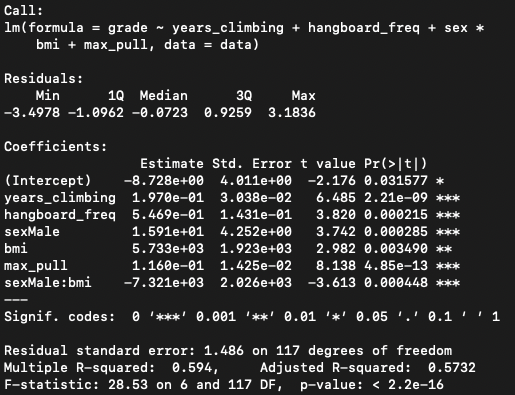
\includegraphics[width=0.7\textwidth]{start}
\end{center}

%%%%%%%%%%%%%%% BASE MODEL DIAGNOSTICS 
\newpage
{\bf\large Initial Assumption Evaluation}\\
Our normality of residuals assumption is holding quite well as displayed by our histogram and q-q plot.\\

\begin{center}
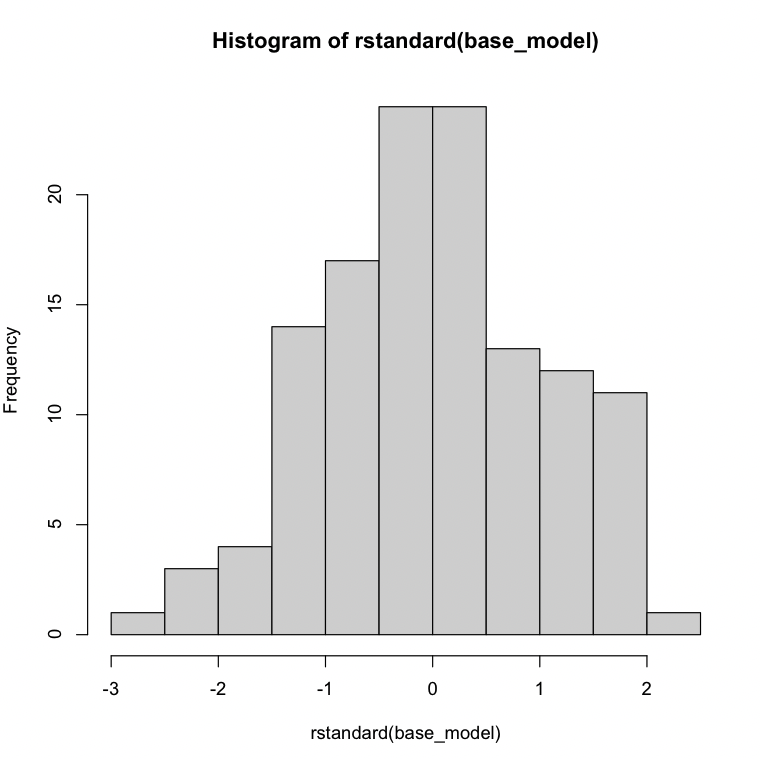
\includegraphics[width=0.6\textwidth]{hist_base}
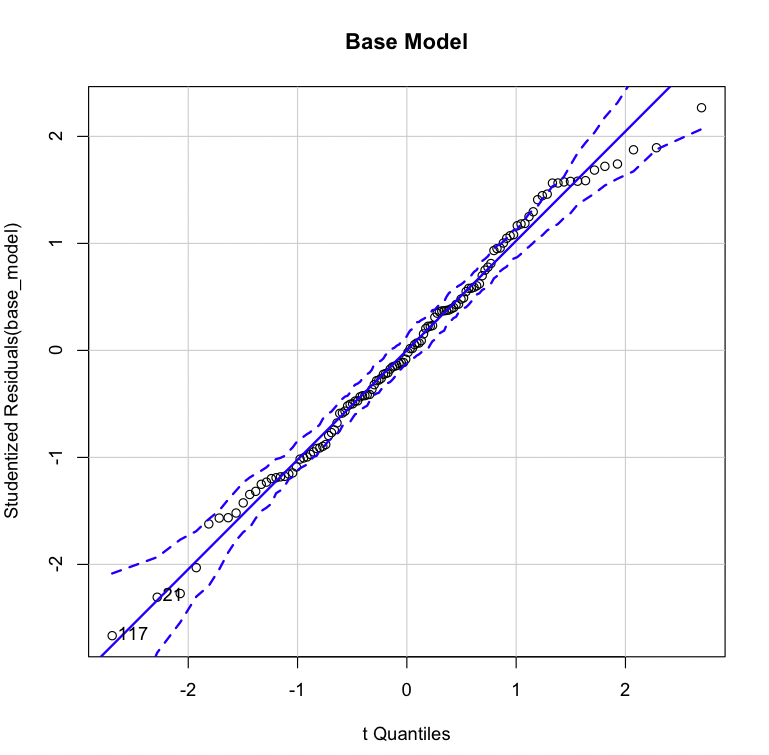
\includegraphics[width=0.6\textwidth]{base_qq}
\end{center}

Additionally the Shapiro-Wilkes test reports a p-value of $0.4226$ which supports the assumption of normality.\\

\newpage
{\bf\large Initial Assumption Evaluation Continued}\\
Next we look at our linearity and homoscedasticity assumption. First observe the residuals plots against each predictor in our model\\

\begin{center}
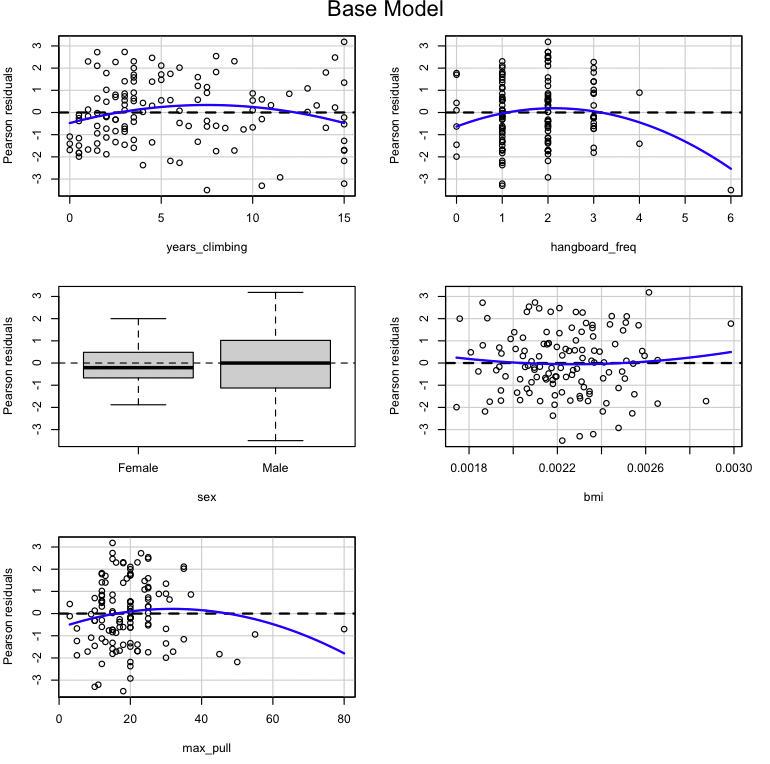
\includegraphics[width=0.5\textwidth]{base_resid}
\end{center}

The plots above suggest that we may be able to improve our linearity assumption of the model via transformations of the max pull up reps and hangboard frequency predictors.
Additionally, there is one potential violation of constant variance in our set of predictors, specifically in years climbing.
There isn't an obvious funnel shape to the residuals when look at the plot, but there are fewer residuals close to zero as years climbing increases. This subtle violation will become apparent when we attempt a log transformation to this variable.
But one should note that this makes a lot of sense because some climbers plateau while others excel.\\

Next observe the residual verse fitted value plots shown below\\

\begin{center}
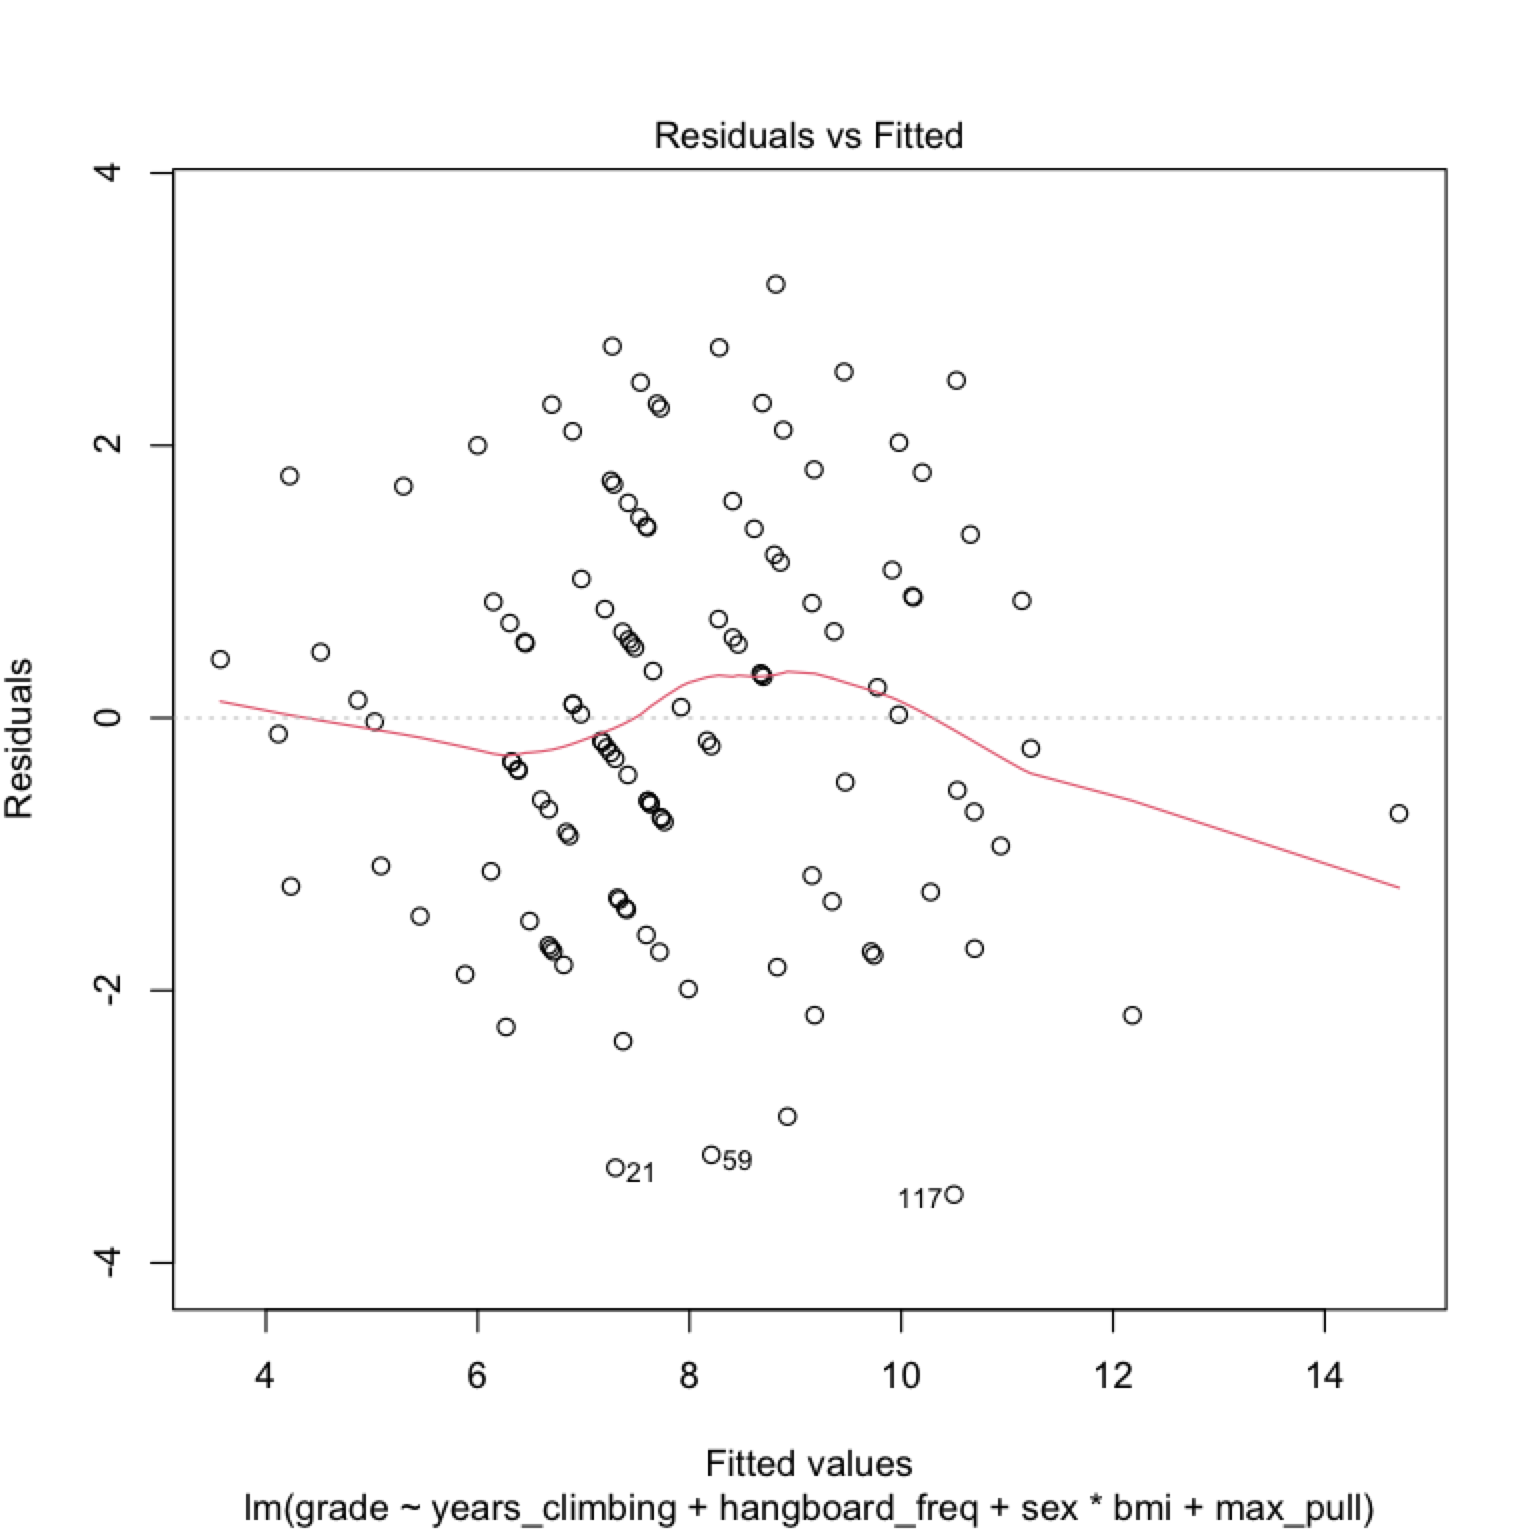
\includegraphics[width=0.3\textwidth]{base_resid_fitted}
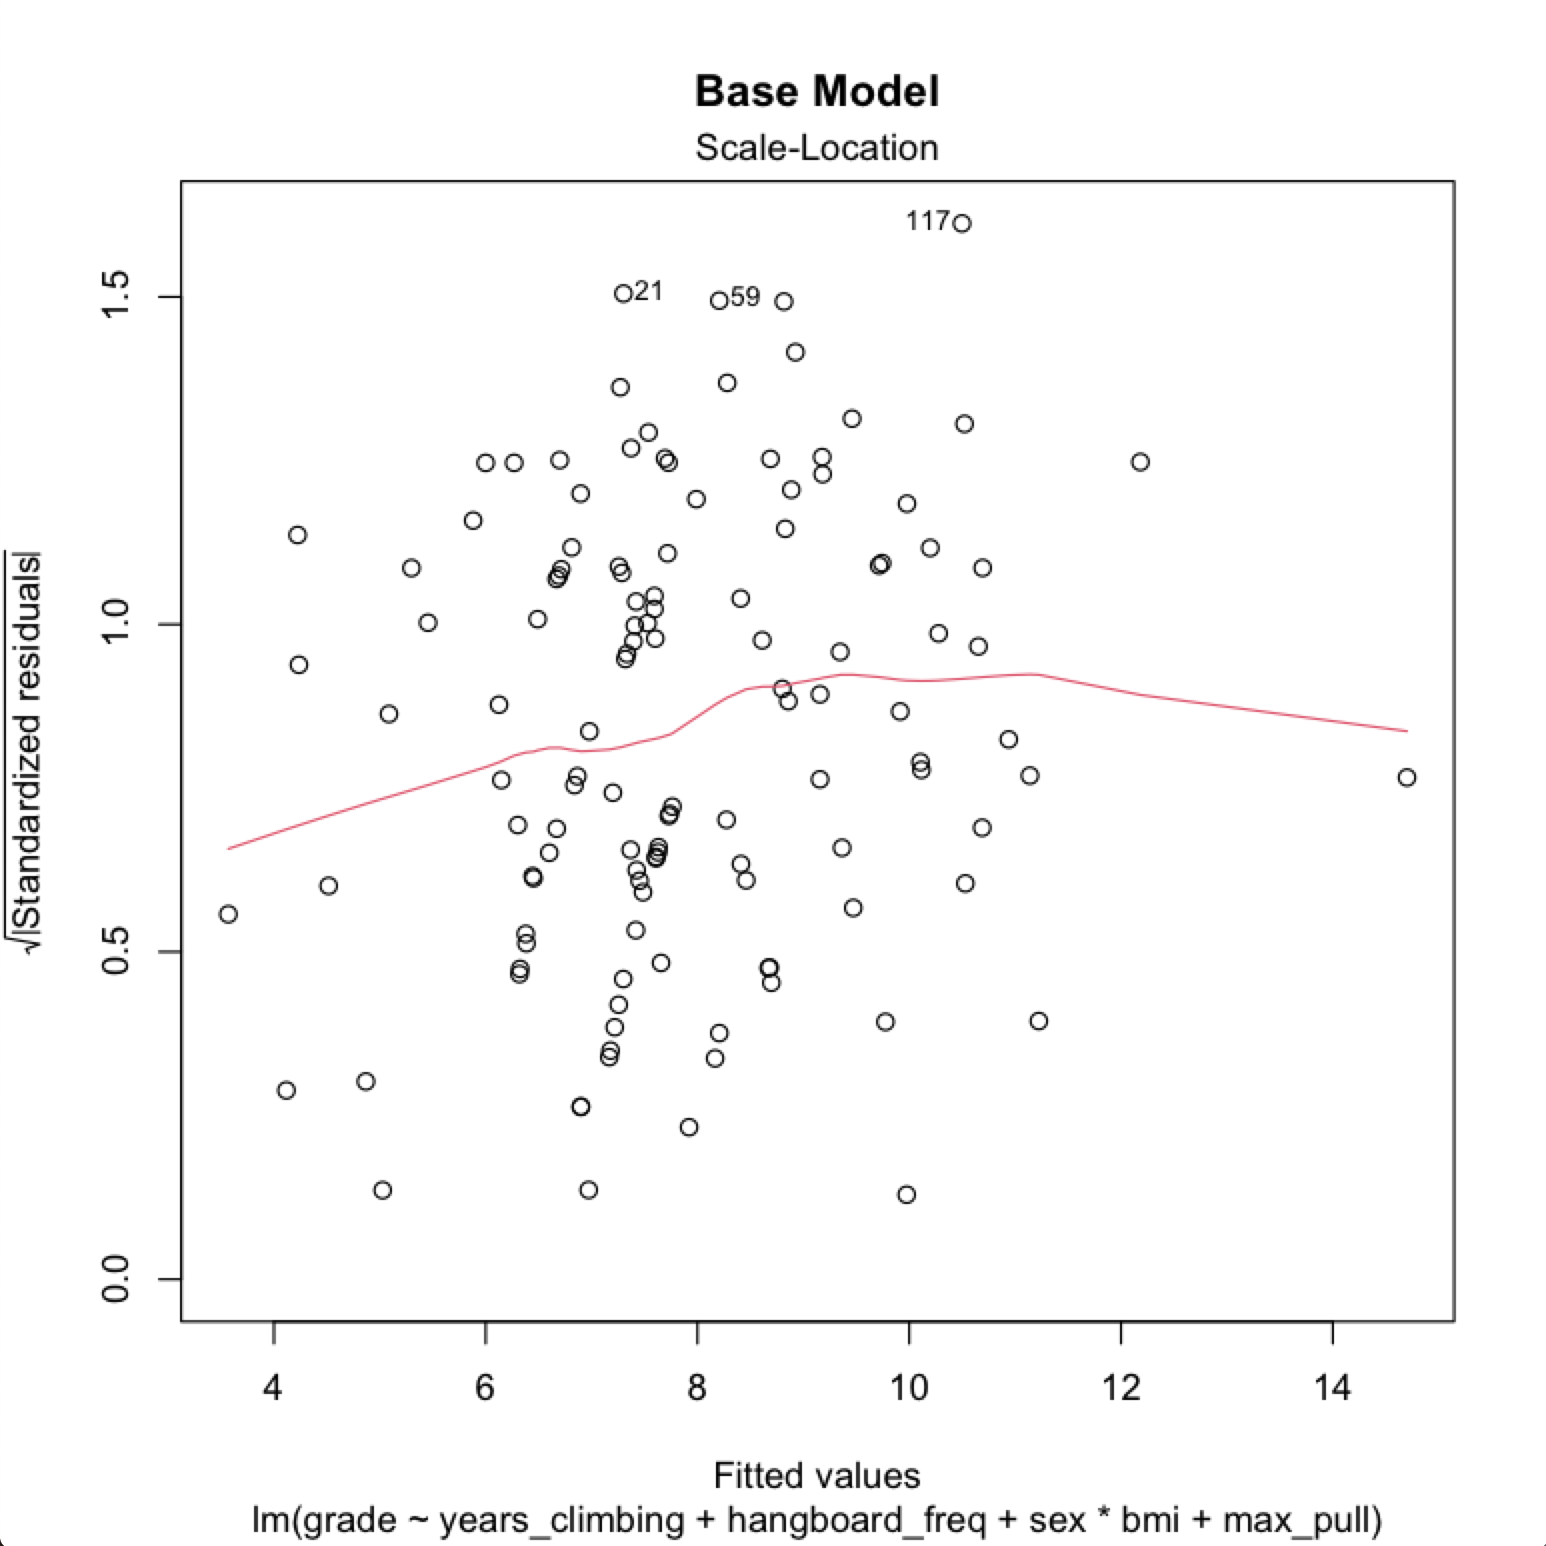
\includegraphics[width=0.3\textwidth]{base_scale}
\end{center}

When looking at the scale location it is evident that our standardized residuals are getting slightly larger as the fitted values increase, which is evidence to suggest that our constant variance assumption is violated.
When viewing the left hand side plot, we see a slight decrease to the trend line for larger fitted values.
This implies we are having some issues modeling elite climbers and in violation of our linearity assumption.
Note, this was also apparent when we looked at residuals verses hangboard frequency and max pull up rep predictors.\\

In summary, the more pressing matter is to deal with issues of model misspecification.
After finding a better model, we will reassess our constant variance assumption. 

%%%%%%%%%%%%%% DATA EXPLORATION
\newpage
{\bf\large Revisiting Initial Data Exploration}\\
By analyzing the scatter plot matrix of our entire data set the following observations occurs:\\

\tab 1. If hangboard frequency is a good predictor, then climbing sessions certainly should be better\\
\tab 2. Max push seems to have a linear relationship with grade but the reciprocal of max push looks even better.\\
\tab 3. Similarly we might try to transform max pull by raising it to the power of $-1$ or $-0.5$. \\
\tab 4. Lack of observations of years climbing in upper left of plot may suggest a log transform is needed\\

The scatter plot matrix is not included in this report due to it's size. However, it can be found in Rplots.pdf upon running the prog4.R script.

\vspace{0.3in}
{\bf\large Addition of Climbing Sessions}\\
It is evident that there is a trend between climbing sessions and hardest grade - a rather good one.
This should have been identified earlier, nonetheless, the new model summary is shown below.\\
 
\begin{center}
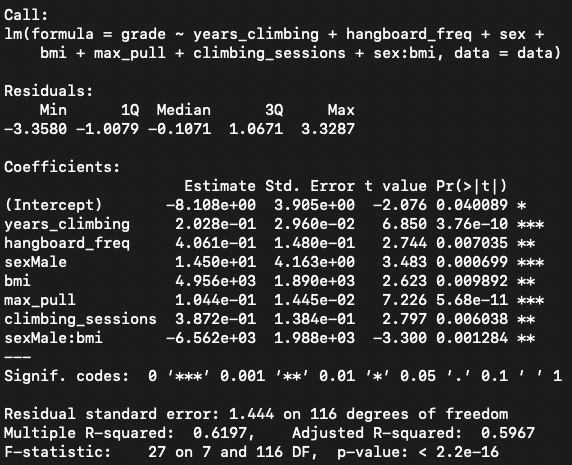
\includegraphics[width=0.5\textwidth]{mod1}\\
\end{center}
 
As you can see, the addition of this new predictor reduced $\hat\sigma$ and increased both $R^2$ and the adjusted-$R^2$.
For further confirmation, an analysis of variance between the two models reports a rather significant p-value as shown below.

\begin{center}
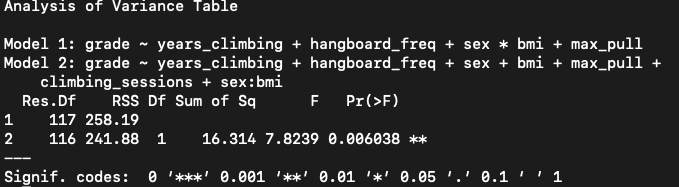
\includegraphics[width=0.5\textwidth]{anova1}
\end{center}

For breavity, I will not perform another diagnostic analysis on this new model but the plots are included in my script (titled "Base Model Plus Climbing Sessions").
The addition of this predictor did not address the previously identified linearity issues.
There where slight improvements to the flattening of the trend-line in the scale-location plot, which suggests an improvement in our assumption that our residuals originate from a population of constant variance.
To support this conclusion, I performed a Breusch-Pagan test on the two models and the p-value increased from $0.18$ to $0.36$
Lastly, the relationship between climbing sessions and hardest grade is rather linear.
There is no evidence to suggest that a transformation of this variable is needed to improve its linear relationship with our response variable.\\

This will be our new working model to try and address the still prevailing linearity issues through data transformations.
We will be referring to it as "the working model" from now on. 

\newpage
{\bf\large Transformation of Max Pull Up Reps}\\
To guide us towards an elegant transformation of the max pull up rep predictor we consider the invTranPlot.
\begin{center}
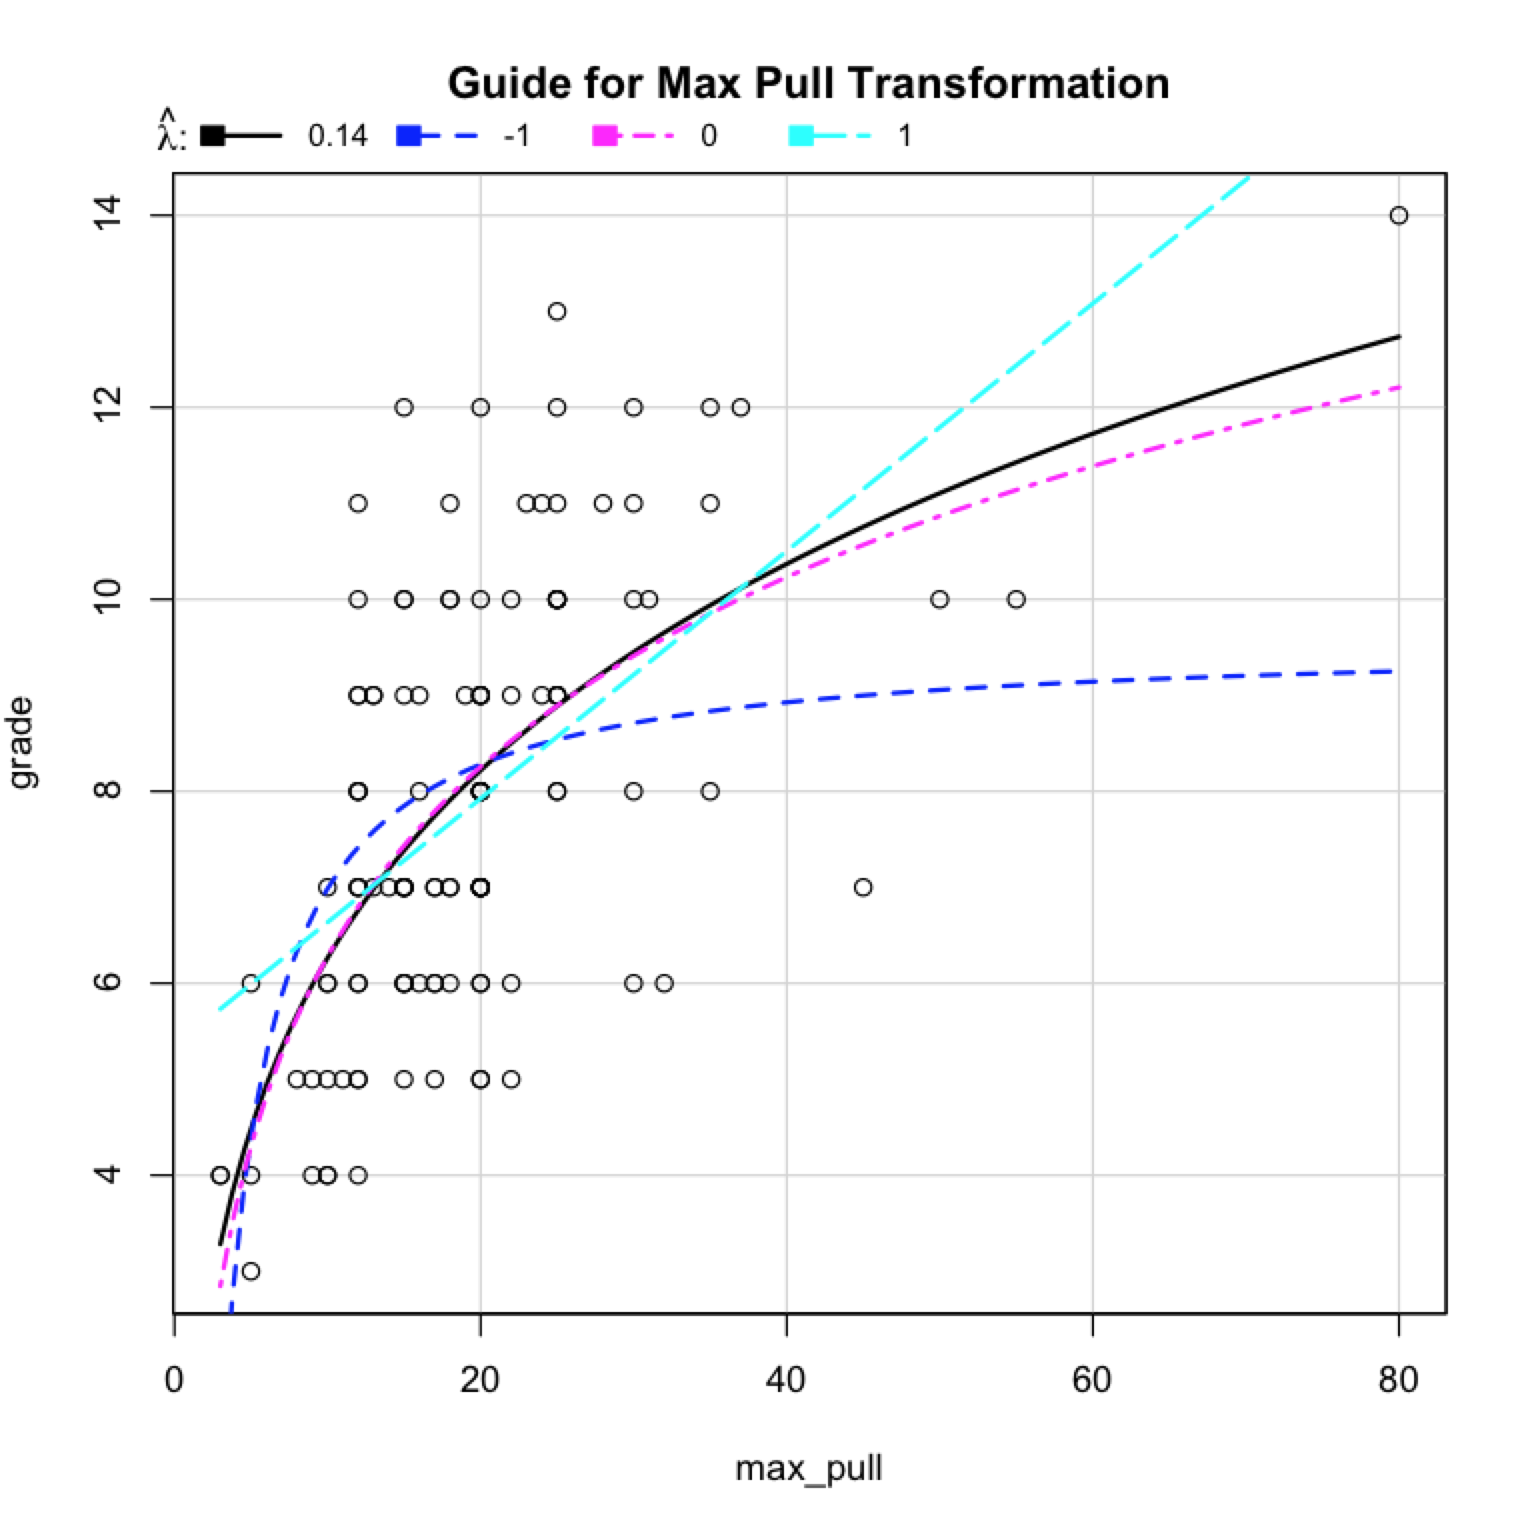
\includegraphics[width=0.5\textwidth]{tran1}
\end{center}
Note that a $\hat\lambda$ so close to $0$ suggests that we should consider a log transformation.
Below is the summary of applying such transformation to our working model.\\

\begin{center}
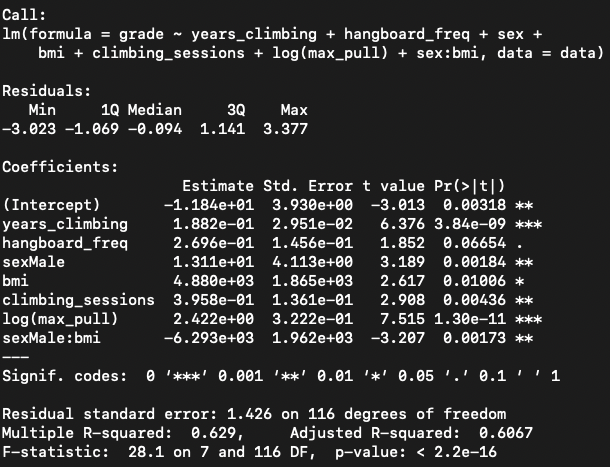
\includegraphics[width=0.5\textwidth]{tran_mod1}
\end{center}

This model certainly provides us with more explanatory power.
However, there is a substantial loss in significance of the hangboard frequency coefficient.
We will be sticking with the rule of dropping any terms that have a p-value greater than .1, so for now it stays.
However, this predictor showed signs of linearity violations thus a better treatment of it in our model may yield the lost significance.



\newpage
{\bf\large Transformation of Max Pull Up Reps Continued}\\
Next we perform a brief diagnostic check to ensure that this transformation did'nt grossly violate any of our assumptions.
The associated plots can be found in Rplots.pdf under the title "Working Model (Transformation of Max Pull)".
However, we do show the residual plots below.

\begin{center}
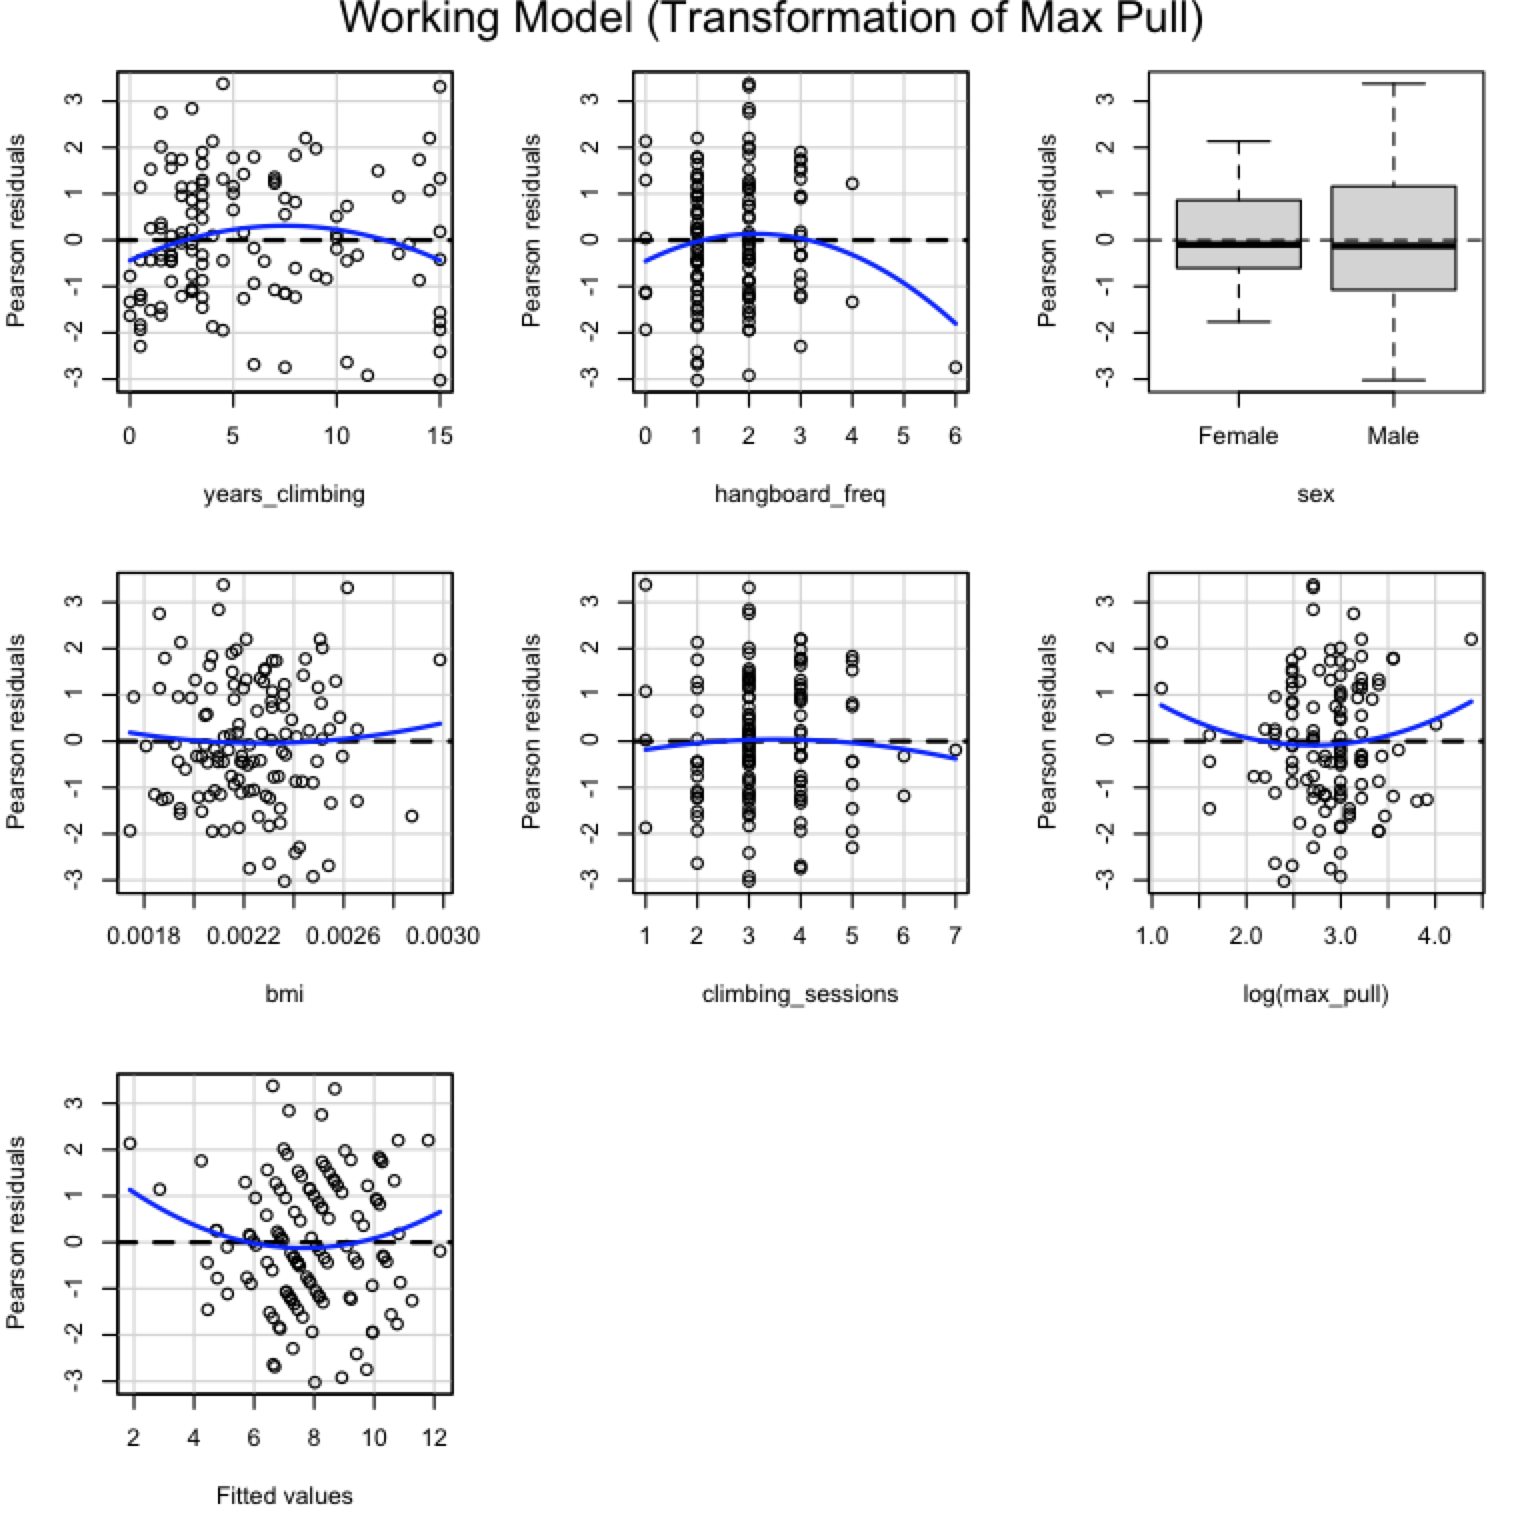
\includegraphics[width=0.5\textwidth]{working_resid1}
\end{center}

As you can see the linearity violation between hardest grade and max pull up reps has indeed improved.
This is probably the best we can hope for and this model will be our new working model.


\vspace{0.3in}
{\bf\large Transformation of Years Climbing (Final Transformation)}\\
To guide us towards an elegant transformation of the years climbing predictor we consider the invTranPlot.
However, since we are using the lower bound of the categorical intervals to treat this predictor numerically - the value $0$ occurs in our data.
Thus, we must shift it horizontally by one unit to the right. 
\begin{center}
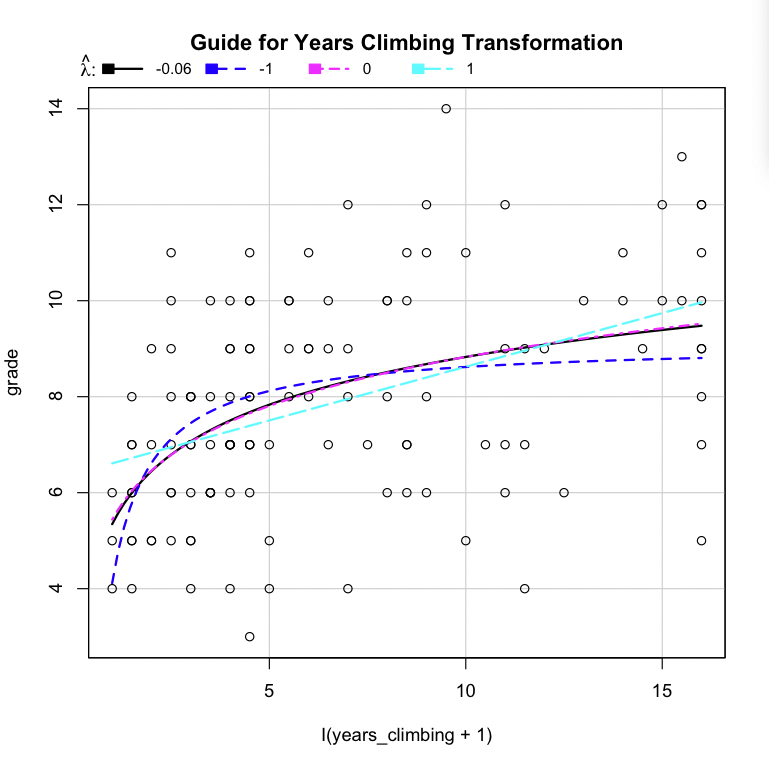
\includegraphics[width=0.45\textwidth]{tran2}
\end{center}
Note this $\hat\lambda$ is even closer to $0$, suggesting that we should consider a log transformation on years climbing plus 1 - because log$(0) = -\infty$, so $0$ can not be an element of years climbing.

\newpage
{\bf\large Transformation of Years Climbing Continued}\\
Below is the summary of applying such transformation to our working model\\

\begin{center}
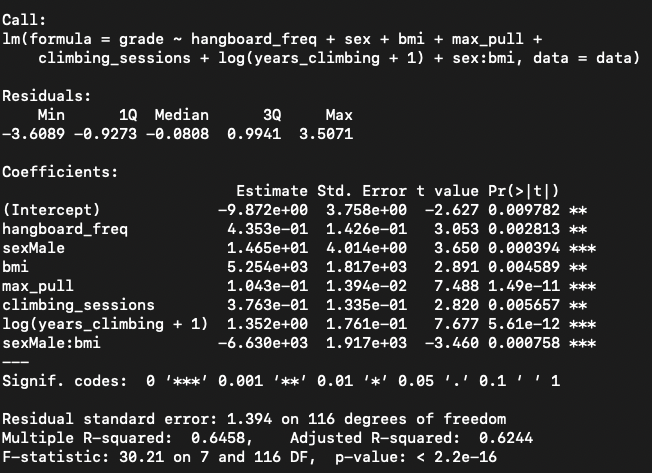
\includegraphics[width=0.5\textwidth]{tran_mod2}
\end{center}

Note that the effect of this transformation definitely increased the explanatory value of our model. Additionally, I find it quite interesting that it restored some of the significance to the hangboard frequency coefficient. This is the inherent issue of trusting such p-values when in violation of our standard assumptions.\\

\begin{center}
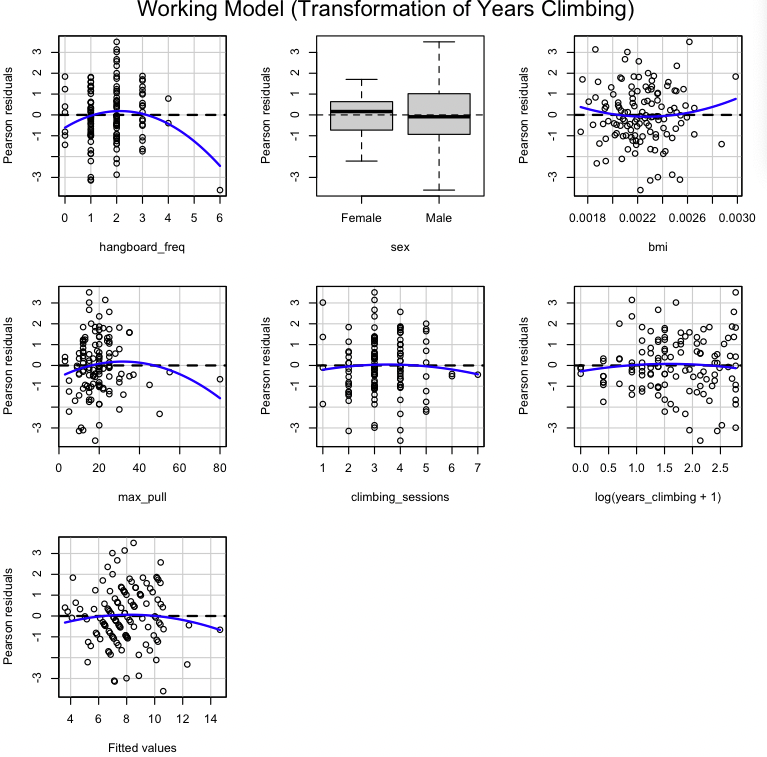
\includegraphics[width=0.5\textwidth]{working_resid2}
\end{center}

Our issue of linearity on the predictor of years climbing is certainly solved.
However, this sheds much light onto the non constant variance issue between years climbing and hardest grade - as shown by the obvious funnel in the plot. This will be investigated in our final conclusion.\\

Note that I have investigated max push up reps inclusion, with and without transformations, and at various stages of the model. It appears to be quite collinear with other predictors.
Therefore, it never found a place in the final model.
Additionally, I have tried various transformations on hangboard frequency and they all drastically reduce the explantory power and significance of it's coefficient. Therefore it remains as is and plays a role in our model.

\newpage
{\bf\large Conclusion and More Diagnostics of Transformed Model}\\
Note that our adjusted-$R^2$ increased by $0.0512$ units while $R^2$ increased by $0.0519$ units, with only a loss of one degree of freedom.
Consequently, our estimate of the standard deviation of our population also improved - from $1.486$ to $1.394$.
It should be noted that our final model has no overly influential observations, though some outliers.
We are in much better standing with all of our assumptions.
The normality of residuals has improved as displayed by our updated qq-plot

\begin{center}
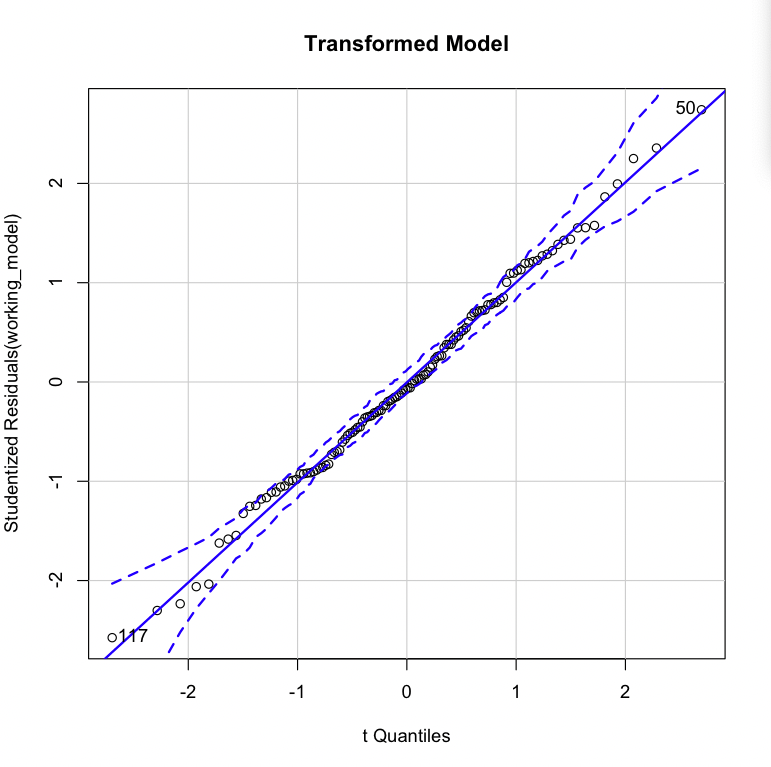
\includegraphics[width=0.45\textwidth]{final_qq}
\end{center}

Additonally, the p-value of our Shapiro-Wilkes test nearly doubled to $0.89$.

Our assumption of constant variance appears to be more believable when considering the results of Breusch-Pagan test, which initially had a p-value of $0.18$ and in our final model the test reported a p-value of $0.46$.
Graphically, this is displayed by the smoothing of the trend line in the scale location plot.
It should be noted that there is obviously an issue in assuming that the variance is constant when using years climbing as predictor of hardest grade - as previously discussed in the years climbing transformation section. 



\begin{center}
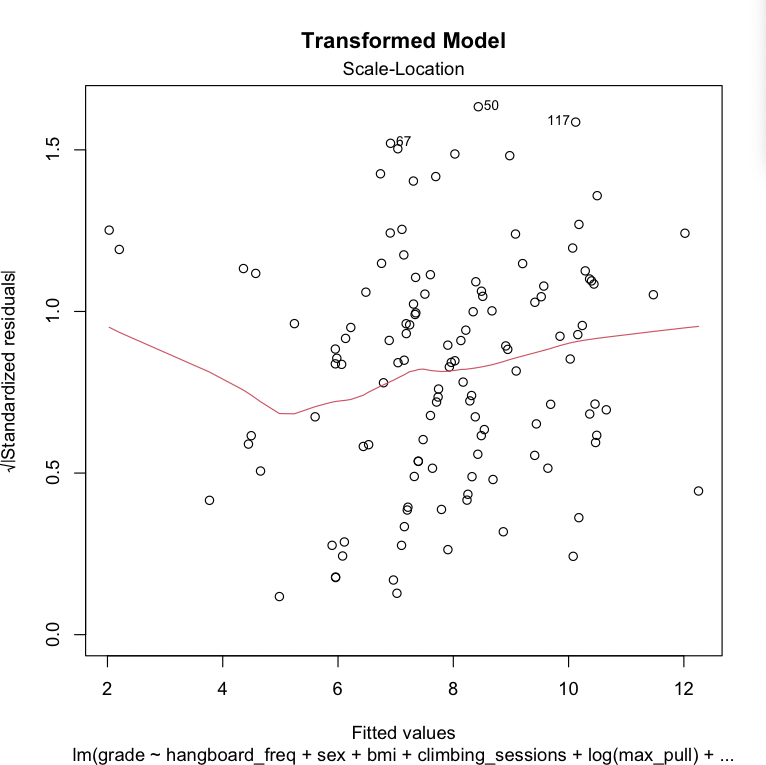
\includegraphics[width=0.45\textwidth]{final_scale}
\end{center}

In conclusion, we made vast improvements to our model misspecification issues via our three transformations.
This is likely the best we can hope for.








\end{document}\\